\documentclass[a4paper]{article}

%figure inside text
\usepackage{wrapfig}

%layout config
\usepackage{calc}
\setlength\textwidth{7in}
\setlength\textheight{10in}
\setlength\oddsidemargin{(\paperwidth-\textwidth)/2 - 1in}
\setlength\topmargin{(\paperheight-\textheight
-\headheight-\headsep-\footskip)/2 - 1in}

%sinuit
\usepackage{siunitx}
%image insertion
\usepackage{graphicx} %image settings
\DeclareGraphicsExtensions{.pdf,.png,.jpg}

%math
\usepackage{amsmath} %math
%\usepackage{cmbright} %math font

%font
\usepackage{kotex}
\usepackage{fontspec}
\ifx가가
\setmainhangulfont[Ligatures=TeX,
BoldFont={KoPubBatang Medium}]{KoPubBatang Light}
\setsanshangulfont[Ligatures=TeX,
BoldFont={KoPubDotum Medium}]{KoPubDotum Light}
\setmainhanjafont[Ligatures=TeX,
BoldFont={KoPubBatang Medium}]{KoPubBatang Light}
\setsanshanjafont[Ligatures=TeX,
BoldFont={KoPubDotum Medium}]{KoPubDotum Light}
\xetexkofontregime[puncts=prevfont, colons=prevfont, cjksymbols=hangul]{latin}
\fi

%줄간격
\usepackage{setspace}
%\usepackage{indentfirst}
\setstretch{1.2}
\everydisplay{\setstretch{1.2}}

%subfigure
\usepackage{subfigure}

\pagestyle{plain}
\title{물리 실험보고서 1}
\author{이한빈, 의예과 2016-13347}

\begin{document}


\numberwithin{equation}{section}
\maketitle

\section{Introduction}
	전하가 자기장 속에서 운동하면 힘을 받는데 그것을 전자기력이라고 하며 다음과 같이 주어진다.
	\begin{equation}
		\vec{F} = q\vec{v} \times \vec{B}
	\end{equation}
	따라서 만약 전하의 운동방향과 자기장이 수직하면 전하가 받는 힘의 크기는 $F=qvB$이고 방향은 오른손법칙에 의해 결정됨을 알 수 있다.

	이 식으로부터 전류가 자기장에 수직한 방향으로 흐르는 도선이 받는 힘을 계산할 수 있는데 $I=Aevn$과 위 식을 연립하면 다음을 얻는다.
	\begin{equation}
		F = BIL
		\label{eq:current}
	\end{equation}
	따라서 자기장을 구할 수만 있으면 전하나 도선이 그 속에서 받는 힘을 알아낼 수 있다.
	
	\begin{figure}[h]
		\centering
		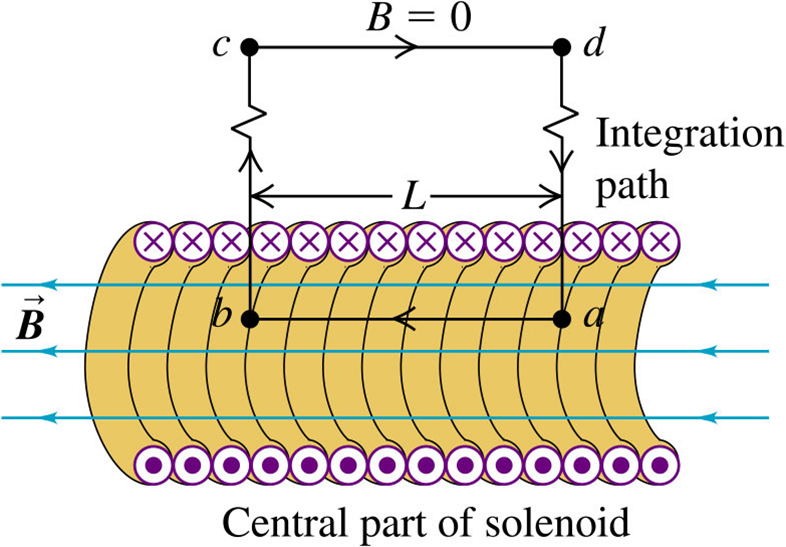
\includegraphics[width=0.4\textwidth]{img/solenoid.png}
		\label{fig:solenoid}
		\caption{솔레노이드와 솔레노이드에 흐르는 전류에 따른 자기장의 방향}
	\end{figure}
	자기장을 발생시키는 장치 중 대표적인 것이 솔레노이드인데 솔레노이드는 원기둥형태로 전선을 일정한 간격으로 감은 장치다.
	솔레노이드의 자기장의 크기는 앙페르 법칙으로 알 수 있으며 그 방향은 그림(\ref{fig:solenoid})처럼 전류방향을 따라 오른손으로 감았을 때 엄지손가락이 가리키는 방향과 같다.

	앙페르 법칙은 흐르는 전류가 만들어내는 자기장을 구할 때 쓰는 식으로 다음과 같이 주어진다.
	\begin{equation}
		\oint \vec{B} \cdot d\vec{s} = \mu{}_{0}I
	\end{equation}

	앙페르 법칙을 이용하여 솔레노이드 내부의 자기장을 구하기 위해 앙페르 폐곡선을 그림(\ref{fig:solenoid})처럼 설정하자.
	폐곡선의 가로길이를 L, 폐곡선을 통과한 전선의 갯수를 N, 솔레노이드 내부의 자기장을 B라고 두면 경로 bc, da의 적분값은 $d\vec{s}$와 $\vec{B}$가 상쇄되어 0이 되고 경로 cd의 적분값은 $B=0$이기 때문에 0이 된다.
	따라서 경로 ab의 적분값만 남게 되어 다음을 얻는다.
	\begin{equation}
		BL = \mu{}_{0}NI
		\label{eq:prosol}
	\end{equation}

	솔레노이드 전선의 간격은 일정하므로 $N/L$은 단위 길이당 감은 전선의 갯수 n과 같음을 알 수 있고 따라서 식(\ref{eq:prosol})의 양변을 L로 나누면 다음을 얻는다.
	\begin{equation}
		B = \mu{}_{0}nI
		\label{eq:sol}
	\end{equation}

	본 실험에서는 솔레노이드와 전류가 흐르는 도선을 이용하여 토크를 발생시키고, 그 토크를 측정함으로써 식(\ref{eq:sol})과 식(\ref{eq:current})을 정량적으로 검증한다.

	\section{Method}
	\vspace{-1cm}
		\begin{figure}[h]
			\centering
			\subfigure[오른쪽 직류이중전원장치 왼쪽 전류천칭]{
			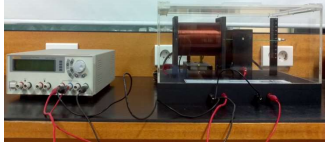
\includegraphics[width=0.4\textwidth]{img/eximg.PNG}
			}
			\subfigure[전류천칭의 회로도]{
			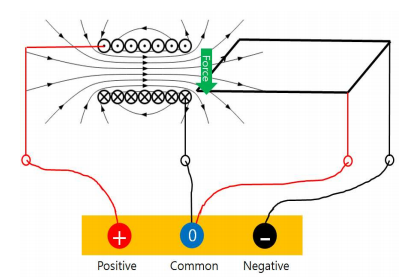
\includegraphics[width=0.4\textwidth]{img/circuit.png}
			\label{fig:circuit}
			}
		\end{figure}
		준비물 : 솔레노이드(길이 12\si{cm}, 감은수 550회), 직류이중전원장치, 집게 전선, 전류 천칭, 마이크로미터
		\subsection{전류천칭의 전류에 따른 토크의 변화}

		\begin{wrapfigure}{r}{0.6\textwidth}
			\centering
            \vspace{-0.5 cm}
			\begin{tabular}{cccccccccc} 
				\hline \hline
				전류(A) \vline & 0.0 & 0.3 & 0.5 & 0.75 & 1.0 & 1.25 & 1.5 & 1.75 & 2.0 \\
				\hline \hline
			\end{tabular}  \vspace{-0.2cm} \caption{천칭에 인가된 전류}
			\vspace{-0.5cm}
			\label{tb:cirinput}
		\end{wrapfigure}
		솔레노이드를 회로도(\ref{fig:circuit})와 같이 되도록 연결했다. 
		전원장치의 전류가 0으로 설정된 것을 확인한 후 전원을 켰다.
		전원장치의 전류와 전압값을 조절하여 천칭의 회로부분이 밑으로 기울어지게 설정했다.
		이때 천칭의 무게 추 쪽 끝이 마이크로미터 기준(가리키게)으로 +0.2\si{cm}가 되도록 했다.
		솔레노이드에 흐르는 전류를 1\si{A}로 고정하고 전류천칭에 흐르는 전류를 표(\ref{tb:cirinput})를 따라 바꿔가며 가리키게의 변위를 측정했다.

		\subsection{솔레노이드의 전류에 따른 토크의 변화}

		\begin{wrapfigure}{r}{0.42\textwidth}
			\centering
            \vspace{-0.5 cm}
			\begin{tabular}{ccccccc} 
				\hline \hline
				전류(A) \vline & 0.0 & 0.5 & 1.0 & 1.5 & 2.0 & 2.5 \\
				\hline \hline
			\end{tabular}  \vspace{-0.2cm} \caption{솔레노이드에 인가된 전류}
			\vspace{-0.5cm}
			\label{tb:solinput}
		\end{wrapfigure}
		솔레노이드를 회로도(\ref{fig:circuit})와 같이 되도록 연결했다. 
		전원장치의 전류가 0으로 설정된 것을 확인한 후 전원을 켰다.
		전원장치의 전류와 전압값을 조절하여 천칭의 회로부분이 밑으로 기울어지게 설정했다.
		이때 천칭의 무게 추 쪽 끝이 마이크로미터 기준(가리키게)으로 +0.2\si{cm}가 되도록 했다.
		전류천칭에 흐르는 전류를 0.5\si{A}로 고정하고 솔레노이드에 흐르는 전류를 표(\ref{tb:solinput})를 따라 바꿔가며 가리키게의 변위를 측정했다.
	
	\section{Result}
		\subsection{전류천칭의 전류에 따른 토크의 변화}
		\begin{figure}[h]
			\centering
          
			\begin{tabular}{cccccccccc} 
				\hline \hline
				전류(\si{A})   \qquad \qquad \vline & 0.0 & 0.3 & 0.5 & 0.75 & 1.0 & 1.25 & 1.5 & 1.75 & 2.0 \\
				\hline
				가리키게 눈금(\si{cm}) \vline & 9.9 & 9.9 & 9.9 & 9.9 & 9.9 & 10 & 10 & 10 & 10 \\
				\hline
				가리키게 변위(\si{cm}) \vline & 0.2 & -0.0 & -0.1 & -0.4 & -0.6 & -0.8 & -1.2 & -1.4 & -1.7 \\
				\hline \hline
			\end{tabular}  \vspace{-0.2cm} \caption{천칭에 인가된 전류와 그에 따른 가리키게의 길이와 위치의 변화}
			\vspace{-0.5cm}
			\label{tb:cirouput}
		\end{figure}
		
		\subsection{솔레노이드의 전류에 따른 토크의 변화}
		\begin{figure}[h]
			\centering
				\begin{tabular}{cccccc} 
					\hline \hline
					전류(A) \qquad \qquad \vline & 0.5 & 1.0 & 1.5 & 2.0 & 2.5 \\
					\hline
					가리키게 눈금(\si{cm}) \vline & 9.9 & 9.9 & 9.9 & 10.0 & 10.5 \\
					\hline
					가리키게 변위(\si{cm}) \vline & -0.5 & -0.9 & -1.3 & -1.8 & -2.4 \\
					\hline \hline
				\end{tabular}  \vspace{-0.2cm} \caption{솔레노이드에 인가된 전류와 그에 따른 가리키게의 길이와 위치의 변화}
			\vspace{-0.5cm}
			\label{tb:soloutput}
		\end{figure}
\newpage

	지막으로 자석의 크기가 클수록 전동기에 인가된 전류와 전압이 클수록 유도기전력의 크기가 커짐을 알 수 있었다. 전동기에 인가된 전류와 전압이 클수록 회전 속도가 빨라진다는 사실로부터 이 결과가 식 (\ref{eq:period})와 잘 일치함을 알 수 있다.



\section{Reference 및 부록}
	1. Halliday, D., Resnick, R., \& Walker, J. (2014). {\it{}Principles of Physics} (10th ed., Vol. 2). Hoboken, NJ: Wiley.
	\\ 

\end{document} 

%실험에서 개선할 점 등 피피티에서 봤던 거 모두 적어서 처리합시다